\documentclass[tikz,border=6pt]{standalone}
% Shared style for the HERMESS schematic figures (compiled by build.sh).
% ETH palette; Latin Modern (the LaTeX default) to match the documentation.
\usepackage{amsmath}
\usepackage{tikz}
\usetikzlibrary{arrows.meta,positioning,calc,shapes.geometric,circuits.ee.IEC}
\definecolor{ethblue}{HTML}{215CAF}
\definecolor{ethpetrol}{HTML}{007894}
\definecolor{ethgrey}{HTML}{6F6F6F}
\tikzset{
  block/.style      = {draw=ethblue, thick, fill=ethblue!8, minimum height=9mm,
                       minimum width=16mm, inner sep=2.5pt, align=center},
  sum/.style        = {draw=ethblue, thick, circle, fill=white, minimum size=4.5mm, inner sep=0pt},
  sig/.style        = {-{Latex[length=2.4mm]}, thick},
  wire/.style       = {thick},
  node distance     = 9mm and 12mm,
  every node/.style = {font=\small},
  lbl/.style        = {font=\small, inner sep=1.5pt},
  port/.style       = {font=\small\itshape, text=ethgrey},
}

\begin{document}
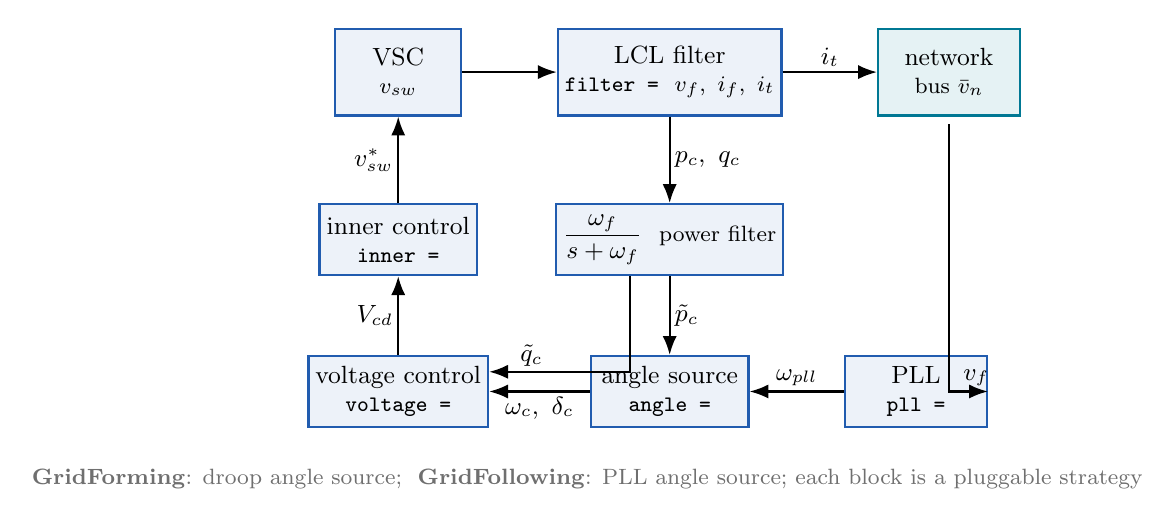
\begin{tikzpicture}[node distance=8mm and 12mm]
  % power path
  \node[block, minimum width=16mm, minimum height=11mm] (vsc) {VSC\\[-1pt]{\footnotesize $v_{sw}$}};
  \node[block, right=12mm of vsc, minimum width=26mm, minimum height=11mm] (lcl) {LCL filter\\[-1pt]{\footnotesize\texttt{filter =}\ \ $v_f,\ i_f,\ i_t$}};
  \node[block, right=12mm of lcl, minimum width=18mm, minimum height=11mm, fill=ethpetrol!10, draw=ethpetrol] (grid) {network\\[-1pt]{\footnotesize bus $\bar v_n$}};
  \draw[sig] (vsc) -- (lcl);
  \draw[sig] (lcl) -- (grid) node[midway, above, lbl] {$i_t$};
  % measurement filter
  \node[block, below=11mm of lcl, minimum width=26mm] (meas) {$\dfrac{\omega_f}{s + \omega_f}$\ \ {\footnotesize power filter}};
  \draw[sig] (lcl) -- (meas) node[midway, right, lbl] {$p_c,\ q_c$};
  % control blocks
  \node[block, below=11mm of vsc, minimum width=20mm] (inner) {inner control\\[-1pt]{\footnotesize\texttt{inner =}}};
  \node[block, below=10mm of inner, minimum width=20mm] (volt) {voltage control\\[-1pt]{\footnotesize\texttt{voltage =}}};
  \node[block, below=10mm of meas, minimum width=20mm] (angle) {angle source\\[-1pt]{\footnotesize\texttt{angle =}}};
  \node[block, right=12mm of angle, minimum width=18mm] (pll) {PLL\\[-1pt]{\footnotesize\texttt{pll =}}};
  \draw[sig] (meas) -- (angle) node[midway, right, lbl] {$\tilde p_c$};
  \draw[sig] ($(meas.south)+(-0.5,0)$) |- ($(volt.east)+(0,0.25)$) node[pos=0.85, above, lbl] {$\tilde q_c$};
  \draw[sig] (angle.west) -- (volt.east) node[midway, below, lbl] {$\omega_c,\ \delta_c$};
  \draw[sig] (volt) -- (inner) node[midway, left, lbl] {$V_{cd}$};
  \draw[sig] (inner) -- (vsc) node[midway, left, lbl] {$v_{sw}^{*}$};
  \draw[sig] ($(grid.south)+(0,-0.1)$) |- (pll.east) node[pos=0.85, above, lbl] {$v_f$};
  \draw[sig] (pll) -- (angle) node[midway, above, lbl] {$\omega_{pll}$};
  \node[lbl, text=ethgrey] at ($(volt.south)+(2.4,-0.65)$)
    {\footnotesize \textbf{GridForming}: droop angle source;\ \ \textbf{GridFollowing}: PLL angle source; each block is a pluggable strategy};
\end{tikzpicture}
\end{document}
